\section{Arbol B}

\subsection{investigar una función para árboles b en python}

\subsubsection{Funciones básicas:}

\begin{itemize}
  \item Insertar(clave): Inserta una nueva clave en el árbol.
  \item Eliminar(clave): Elimina una clave del árbol.
  \item Buscar(clave): Busca una clave en el árbol y devuelve True si la encuentra o False si no la encuentra.
  \item Recorrer(orden): Recorre el árbol en un orden determinado (inorden, preorden o postorden).
\end{itemize}

\subsubsection{Funciones avanzadas:}

\begin{itemize}
  \item Altura(): Devuelve la altura del árbol.
  \item Tamaño(): Devuelve el número de nodos del árbol.
  \item Balancear(): Equilibra el árbol para que sea lo más eficiente posible.
  \item Dividir(nodo): Divide un nodo en dos nodos hijos.
  \item Unir(nodo1, nodo2): Une dos nodos hijos en un solo nodo padre.
  \item Bibliotecas para árboles B en Python:
\end{itemize}

\subsubsection{Bibliotecas para árboles B en Python:}

\begin{itemize}
  \item bintrees: Implementación simple y eficiente de árboles B en Python.
  \item bbolt: Biblioteca para bases de datos NoSQL que utiliza árboles B como estructura de datos subyacente.
  \item btree: Implementación de árboles B en Python con soporte para transacciones.
\end{itemize}


\subsection{leer cada palabra del archivo de animales e ir insertando en un árbol b de grado 4.}

\subsubsection{Leer el archivo:}

\begin{itemize}
  \item Se abre el archivo animales.txt en modo lectura.
  \item Se recorre cada línea del archivo.
  \item Se elimina cualquier espacio en blanco al principio y al final de cada línea.
\end{itemize}

\subsubsection{Insertar la palabra en el árbol B:}
\begin{itemize}
  \item Se verifica si la palabra ya está en el árbol B.
  \item Si la palabra no está en el árbol B, se busca la posición donde debería insertarse.
  \item Se inserta la palabra en la posición correcta.
  \item Si la inserción provoca que un nodo tenga más de 4 claves, se divide el nodo en dos nodos hijos.
\end{itemize}

\subsubsection{Repetir los pasos 1 y 2 para cada palabra del archivo:}
\begin{itemize}
  \item Se continúa leyendo el archivo línea por línea.
  \item Se inserta cada palabra en el árbol B.
  \item Se continúa dividiendo los nodos que tengan más de 4 claves.
\end{itemize}

\subsubsection{El árbol B final contendrá todas las palabras del archivo:}
\begin{itemize}
  \item Cada palabra estará en una única posición del árbol B.
  \item Las palabras estarán ordenadas en el árbol B.
  \item El árbol B tendrá un grado de 4, lo que significa que cada nodo tendrá como máximo 4 claves y 5 hijos.
\end{itemize}


\subsection{mostrar en consola el árbol.}

\begin{figure}[ht]
  \centering
  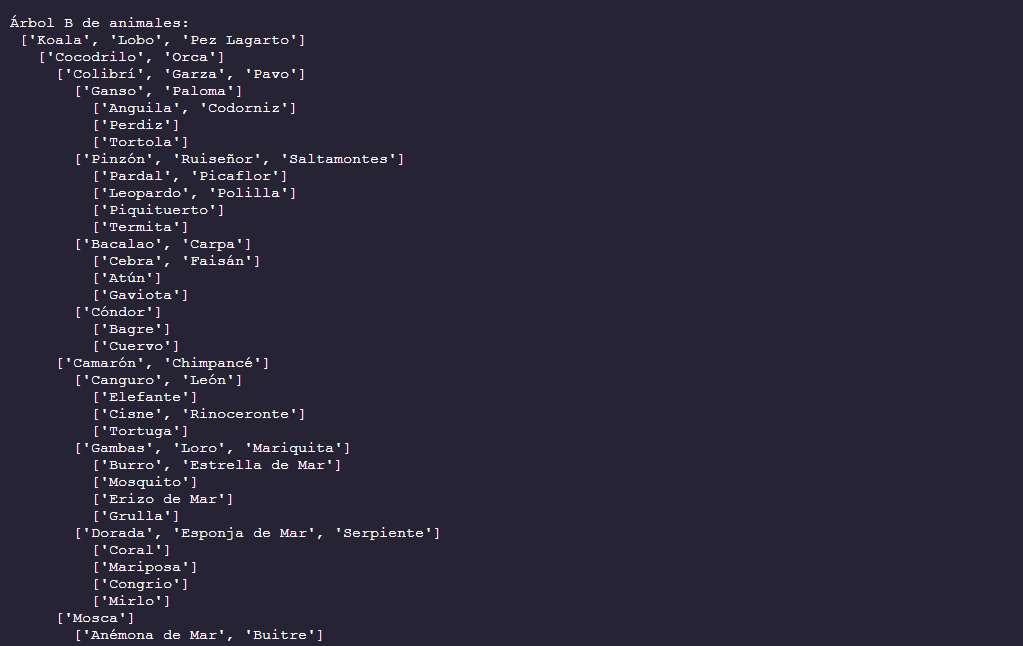
\includegraphics[width=0.7\textwidth]{./src/img/arbol/image1.png}
\end{figure}

\subsection{realizar una consulta al árbol sobre una palabra que sí exista y otra que no exista y mostrar los resultados}

\begin{figure}[ht]
  \centering
  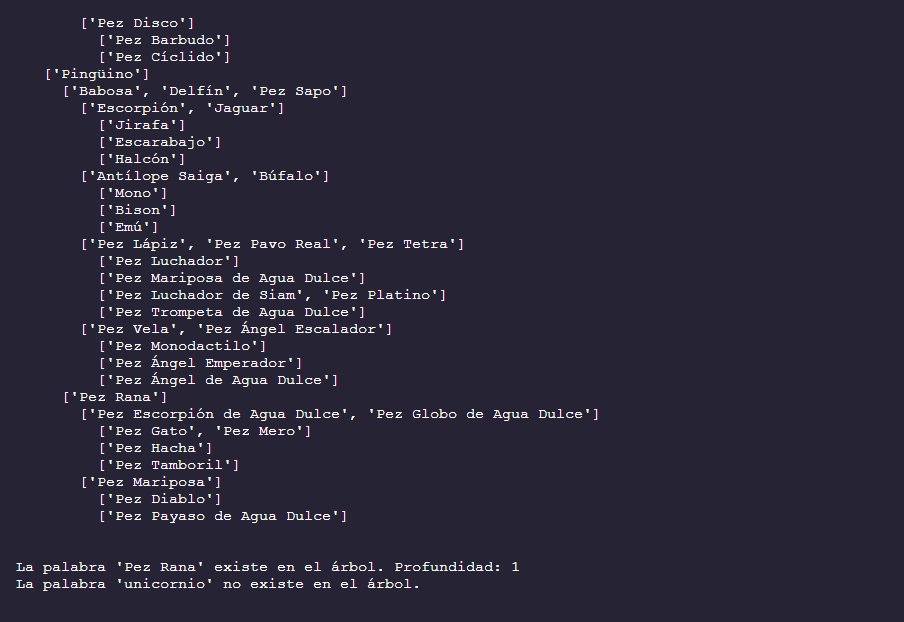
\includegraphics[width=0.7\textwidth]{./src/img/arbol/image2.png}
\end{figure}